%                                             -*- coding: utf-8 -*-
% Mindenkinek csak javasolni tudjuk, hogy latex-et használjon.
% Szakdolgozatnál vagy diplománál már egyértelműen kijönnek az
% előnyei a Worddel szemben.  Ennek ellenére ez a sablon messze nem
% tökéletes.  Ha valamit javítanál benne, kérlek, küld vissza, hogy
% hallgatótársaid is profitáljanak belőle.  Köszönöm.

% További nehézséget okoz, hogy a népszerű latex disztribúciók nem
% tartalmazzák a legújabb változatát a magyar.ldf-nek.  A szükséges
% fájlokat a sablon mellé bemásoltuk, de le is tölthetőek innen:
% http://www.math.bme.hu/latex/
%
%
%
\documentclass[11pt,a4paper,oneside]{article}
\usepackage[margin=3cm]{geometry}
% =================================================================
% Magyar nyelvi támogatás
%------------------------
% ###################
% Nyelvváltó parancsok:
%\selectlanguage{english}
%\selectlanguage{magyar}
% rövid angol beszúrás:  \foreignlanguage{english}{some english text}
% határozott névelők generálása ``magyar'' babel-el:
% argumentum+megfelelő határozott nevelő: \az{},\Az{}
% csak a megfelelő határozott nevelő: \az*{}, \Az*{}
% címkék: \aref{}, \aref*{}, képletekhez \aref()
%        \Aref{}, \Aref*{}, képletekhez \Aref()
% oldalak: \apageref{}, \apageref*{}
%        \Apageref{}, \Apageref*{}
% idézetek: \acite, \acite*, \Acite, \Acite*
% ###################
\usepackage[english]{babel} %vegyes nyelvi támogatás a
% magyar helyesírás ellenőrzéshez (ispell) és elválasztáshoz
\selectlanguage{english}

%=================================================================
% direkt ékezetes karakter beírás támogatás
%-------------------------------------------
\usepackage[T1]{fontenc}
\usepackage[utf8]{inputenc}
\usepackage{multirow} 
%================================================================
% Undorító dolog bitmappelt (Type III) betűtípust nézni a PDF-ben
% képernyőn. Az alapértelmezett Computer Modern font LaTex-ben
% bitmappelt, ezért használjunk Times fontot:
\usepackage{times}

%================================================================
% ha ábrát akarunk beemelni, akkor használjuk a graphicx/graphics
% csomagot és az \includegraphics[width=<width>]{abra.pdf} parancsot
\usepackage{graphicx} %for graphics
%kepek helye a gyokerhez(ehhez a file-hoz kepest) kepest
\graphicspath{{./figs/}}

\usepackage{tabularx}
\usepackage[skip=1ex]{caption}

%================================================================
% Kötelezően használjuk a hyperref csomagot, mert ezzel többek között 
%  kultúrált hyperlinkelt PDF-et lehet csinálni az alábbi
%  variációkban, különféle hyperref backend-ekkel:
%  pdflatex,dvipdfm,ps2pdf
% tapsztalataim szerint a MikTeX (Win32) a 'dvipdfm' konverzióval
% optimális  míg a teTeX (Linux/Solaris) jobb szereti a 'dvips' módszert
%------------------------------------
% pontosan egyet kommentezzünk be!!!!!!!
% értelemszerűen backend függően generáljunk dvi-ból PDF-et!!!
%------------------------------------
% A hyperref csomag az utolsó beolvasott csomag legyen, kivéve néhány
% problémás csomagot, pl. algorithm
%-----------
% ########################### FONTOS ###########################
% A hyperref hibásan működik a babel csomag 'magyar.ldf' fájljának
% 1.5-ös verziójánál korábbi változatával. 2004. februárjában a MikTeX
% és teTex disztribúciók még csak a v.1.4 verziót tartalmazták! A fájl
% aktuális verziója a BME Matematikai intézet LaTeX honlapjáról
% elérhető: http://www.math.bme.hu/latex/ 
% A lusták kedvéért a jelen sablon mellé is mellékelem:
% magyarlatex_0.01-2.tar.gz 
% ########################### FONTOS ###########################
%-----------
\PassOptionsToPackage{hyphens}{url}\usepackage[colorlinks=true]{hyperref}
\def\equationautorefname~#1\null{Equation (#1)\null}
\def\figureautorefname~#1\null{Figure (#1)\null}
\def\tableautorefname~#1\null{Table (#1)\null}

%%%%%%%%%%%%%%%%%%%%%%%%%%%%%%%%%%%%%%%%%%%%%%%%%%%%%%%%%%%%%%%%%%%
% Itt kezdődik maga a dokumentum
%%%%%%%%%%%%%%%%%%%%%%%%%%%%%%%%%%%%%%%%%%%%%%%%%%%%%%%%%%%%%%%%%%
\begin{document}
%%%%%%%%%%%%%%%%%%%%%%%%%%%%%%%%%%%%%%%%%%%%%%%%%%%%%%%%%%%%%%%%%%%
% Ezt ne piszkáld!!!!
%%%%%%%%%%%%%%%%%%%%%%%%%%%%%%%%%%%%%%%%%%%%%%%%%%%%%%%%%%%%%%%%%%%
\pagestyle{myheadings} % legyen fejléc 

\newcommand{\semesterprojecttitle}{
  \begin{center}
    \huge{\textbf{Project Laboratory Report}}
    
    \smallskip
    \small{Department of Telecommunications and Media Informatics}
  \end{center}
  \bigskip
} 

% Argumentumok: #1=Név, #2=Neptunkód, #3=szakirány, #4=email, #5 konzulens-1, #6 konzulens-1-email, #7 konzulens-2, #8 konzulens-2-email
\newcommand{\semesterprojectauthor}[6]{

\begin{center}
  \begin{tabular}{ l c }
  Author:         & \textbf{#1}  \\
  Neptun:         & \textbf{\texttt{#2}}  \\
  Specialization: & \textbf{#3}  \\
  E-mail address: & \href{mailto:#4}{\textbf{#4}}  \\
  Supervisor:     & \textbf{#5}  \\
  E-mail addres:  & \href{mailto:#6}{\textbf{#6}} \\
  
  \end{tabular}
\end{center}
\bigskip

}

% % Argumentumok: #1=Név, #2=email
% \newcommand{\konzulens}[2]{
%   \noindent\textbf{Konzulens:} #1 
%   \newline\emph{Email cím:}\/ \href{mailto:#2}{#2}
%   \newline
% 
% }

% Argumentumok: #1=Tanév (xxxx/xx alakban, #2=félév (pont nélkül)
\newcommand{\semester}[2]{
  \large\textbf{#1 #2. semester}
}

% Argumentumok: #1=téma címe 
\newcommand{\tasktitle}[1]{
  \begin{center}
    \LARGE\textbf{Title: #1}
    \bigskip
  \end{center}
}

% Argumentumok: #1=téma részletei 
\newcommand{\taskdescription}[1]{
\begin{center}
  \Large\textbf{Task} 
\end{center}
#1
\newline
\bigskip
}

% A fejezetek közé beágyazott irod.jegyzék
\def\references#1{\renewcommand{%
\baselinestretch}{1}\list
 {\small [\arabic{enumi}]}{\settowidth\labelwidth{[#1]}\leftmargin\labelwidth
 \advance\leftmargin\labelsep
 \usecounter{enumi}}
 \def\newblock{\small \hskip .11em plus .33em minus .07em}
 \sloppy\clubpenalty4000\widowpenalty4000
 \sfcode`\.=1000\relax}
\let\endreferences=\endlist%


%%% Local Variables: 
%%% mode: latex
%%% TeX-master: "template"
%%% End: 
 % Ez kell!!!
\markright{Márton Torner (OZFKFP)} % egyoldalas fejléc!!!

%--------------------------------------------------------------------
% fedlap
%--------------------------------------------------------------------
\begin{titlepage}
%bme logo 
 \begin{figure}[h]
    \centering
      
\includegraphics[width=12cm]{bme_logo}
  \label{fig:bme_logo}
  \end{figure}
  \thispagestyle{empty}
  %cím generálás
  \semesterprojecttitle
 
  %\author argumentumok: #1=Név, #2=Neptunkód, #3=szakirány, #4=email,#5 konzulens-1, #6 konzulens-1-email, #7 konzulens-2, #8 konzulens-2-email
  \semesterprojectauthor{Márton Torner}{OZFKFP}{Infocommunication (HIT)}{torner.marton@gmail.com}{Bálint Gyires-Tóth, PhD}{toth.b@tmit.bme.hu}
 
 
%\tasktitle argumentuma a task rövid, 1 soros címe
  \tasktitle{Financial time series modeling and forecasting with deep neural networks} 

  %\taskdescription argumentuma a task 1-2 bekezdésnyi ismertetése
  \taskdescription{The task is to collect limit order book data from a chosen crypto exchange, 
  analyze and process the gathered records and to develop a neural network based solution to predict 
  the direction of the price movement of the asset-pairs.
  
  In this work level 100 data (limit order book, depth: 100) is used from Kraken crypto exchange. The live order flow 
  is queried with the help of the provided API and saved on a local storage. The aim is to create a Deep Learning 
  powered system which can predict the price movement direction from the given history. The first approaches are 
  models based on autoregressive solutions (logistic regression and random forest regression) and then I try to use a 
  deep neural network as the model.
  
  In the future this work can be used as a base for creating a complex system for algorithmic trading.}

  %\semester argumentumok:
  % #1=Tanév (xxxx/xx alakban), #2=félév (pont nélkül!)
  \begin{center}
    \semester{2018/19}{II}
  \end{center}
  
\end{titlepage} 

%==================================================================
\begin{center}
  \section{Theory and previous works}
  \label{sec:theory_prev}
\end{center}
% A munka  előzményei és kiindulási állapota
% \newpage
\subsection{Introduction}
\label{sec:introduction}

The computerization of financial markets and the availability of the electronic records of different stock exchanges 
like transactions, order flow and limit order books provide us a great opportunity to analyze and model the dynamics of 
these markets. Over the last years a huge number of studies have been done on this field which can serve as a good base 
for further studies.

With the computerization also came the rapid acceleration of the trading on these financial markets and big companies 
started to use algorithmic solutions to steal a march on their rivals and gain some higher profits.

The quick development that the field of Deep Learning had in the last decade and the impressive number of successful 
researches conducted on the topic of time series forecasting opened the door to change the traditional mathematical 
algorithms with a neural network based solutions. Price forecasting is just a step leading to more complex systems 
which use the predictions as inputs to deliver a trading strategy with the help of machine learning 
(reinforcement learning).

These solutions could change the role of financial specialists in the future.

\subsection{Theoretical summary}
\label{sec:theoretical_summary}

  \subsubsection{Price formation mechanism}
  \label{sec:price_formation_mechanism}
  
  The market price per share of stock (“share price”) is the amount of money an investor is willing to pay to own 
  a company's single stock. The ‘price formation mechanism’ - given in \autoref{eq:price_form} - is a map which tries to 
  represent the relation between market price and different variables affecting it, e.g. price history, order flow, 
  news about the companies or the market etc.

  \begin{equation}
    Price(t+\Delta t) = F(Price history(0...t), Order Flow(0...t), Other Info) = F(X_{t}, \epsilon_{t})
    \label{eq:price_form}
  \end{equation}


  \begin{center}
    \begin{tabular}{l l}
      $X_{t}$: & set of state variables (e.g. order flow, volatility, price, etc.) \\
      $\epsilon_{t}$: & random noise (represents the arrival of new, unknown information) \\
      $\Delta t$: & time resoution
    \end{tabular}
  \end{center}

  \bigskip

  It is shown that this relation is universal (not asset-specific) and stationary (stable across time, even at 
  out-of-sample predictions) ~\cite{univ}. These two features give us the opportunity to use all collected data points 
  to design and train a universal model which can make predictions for all asset-pairs valid even in the future.

  \subsubsection{Limit Order Book}
  \label{sec:limit_order_book}
  
  In this work limit order book data is used as the input so this section tries to provide a short overview what it is 
  and how it works. On stock exchanges we want to buy shares or sell the ones we hold and to accomplish this we place 
  orders of which the LOB consists. There are more special types of orders but in this work only limit orders are used. 
  They remain in the LOB until being executed or cancelled.
  
  The LOB has two sides, the ask and the bid side, shown on \autoref{fig:1}. The ask side represents the sell orders 
  (willing to sell the given amount at the given price) and the bid side the buy orders (willing to buy the given amount 
  at the given price).

  \begin{figure}[tbh]
    \centering
    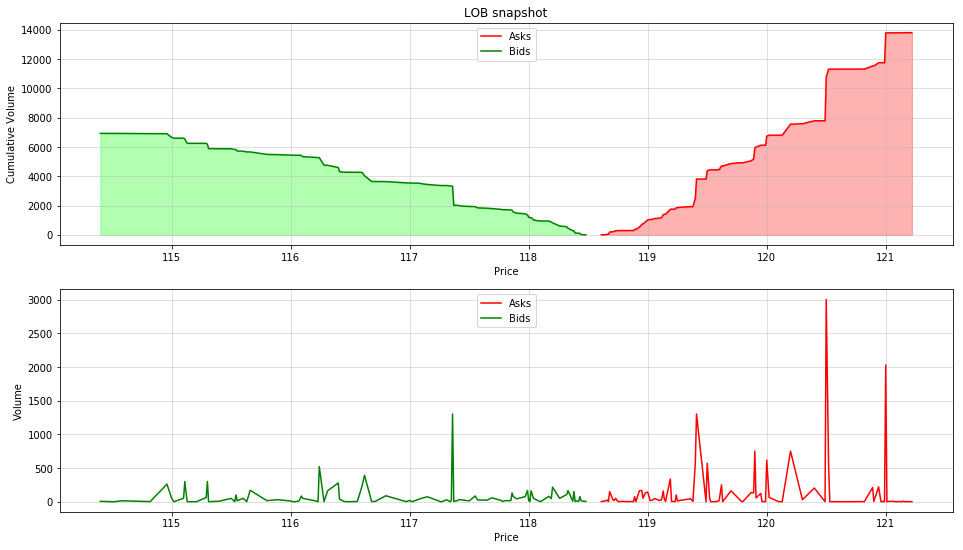
\includegraphics[width=\textwidth]{lob_snapshot.png}
    \caption{Limit Order Book snapshot (ETH\_EUR). Bottom: Volume at each price level. Top: Cumulative volume at price levels.}
    \label{fig:1}
  \end{figure}

  A tick is the measure of the minimum upward or downward movement in a price of a security this means the price levels 
  in the LOB must be the multiples of this value (so order prices can not differ less than this). The best ask price is 
  the lowest sell order and the best bid price is the highest buy order. These are the prices at which the given number 
  of shares can be bought or sold. The difference between best ask and bid price is called the spread and their average 
  is the mid-price (\ref{eq:mid-price}). The weighted average mid-price (WAMP) and volume weighted average price (VWAP) 
  can be calculated as given in \autoref{eq:wamp} and \autoref{eq:vwap}. The depth of the book is used in this paper as 
  the number of best orders on each side (so depth=100 means the top 100 lowest priced ask- and the top 100 highest 
  priced bid orders).

  \begin{equation}
    Mid\-price = \frac{p_{best}^{bid} + p_{best}^{ask}}{2}
    \label{eq:mid-price}
  \end{equation}

  \begin{equation}
    WAMP = \frac{p_{best}^{bid} * v_{best}^{ask} + p_{best}^{ask} * v_{best}^{bid}}{v_{best}^{bid} + v_{best}^{ask}}
    \label{eq:wamp}
  \end{equation}

  \begin{equation}
    VWAP = \frac{(\sum_{i=1}^{depth} (p_i^b * v_i^b))*v^a + (\sum_{i=1}^{depth} (p_i^a * v_i^a))*v^b}{v^a + v^b}
    \label{eq:vwap}
  \end{equation}

  \begin{center}
    \begin{tabular}{l l}
      $p$: & price \\
      $v$: & volume (without lower index = sum over side) \\
      $b$: & bid \\
      $a$: & ask
    \end{tabular}
  \end{center}

  Orders are submitted and cancelled continuously which means that the updates arrive in a very high frequency 
  (millisecond) and it is also easy to see that consuming the order flow of stock exchanges leads to Terabytes of data. 
  At crypto exchanges order manipulation is a big problem to be faced at filtering the collected data. So, to process a 
  live order book we have to deal with various problems [TODO link ide a crawler szekcióhoz].

  \subsubsection{Deep Learning}
  \label{sec:deep_learning}

  Deep Learning models are deep neural networks (an example can be seen on \autoref{fig:2}) trained on large datasets to 
  uncover complex non-linear relations between the (high-dimensional) inputs and outputs. This can be simplified as it 
  represents a functional relation like y = f(x) where y is the output and x is a (high-dimensional) input vector.

  \begin{figure}[tbh]
    \centering
    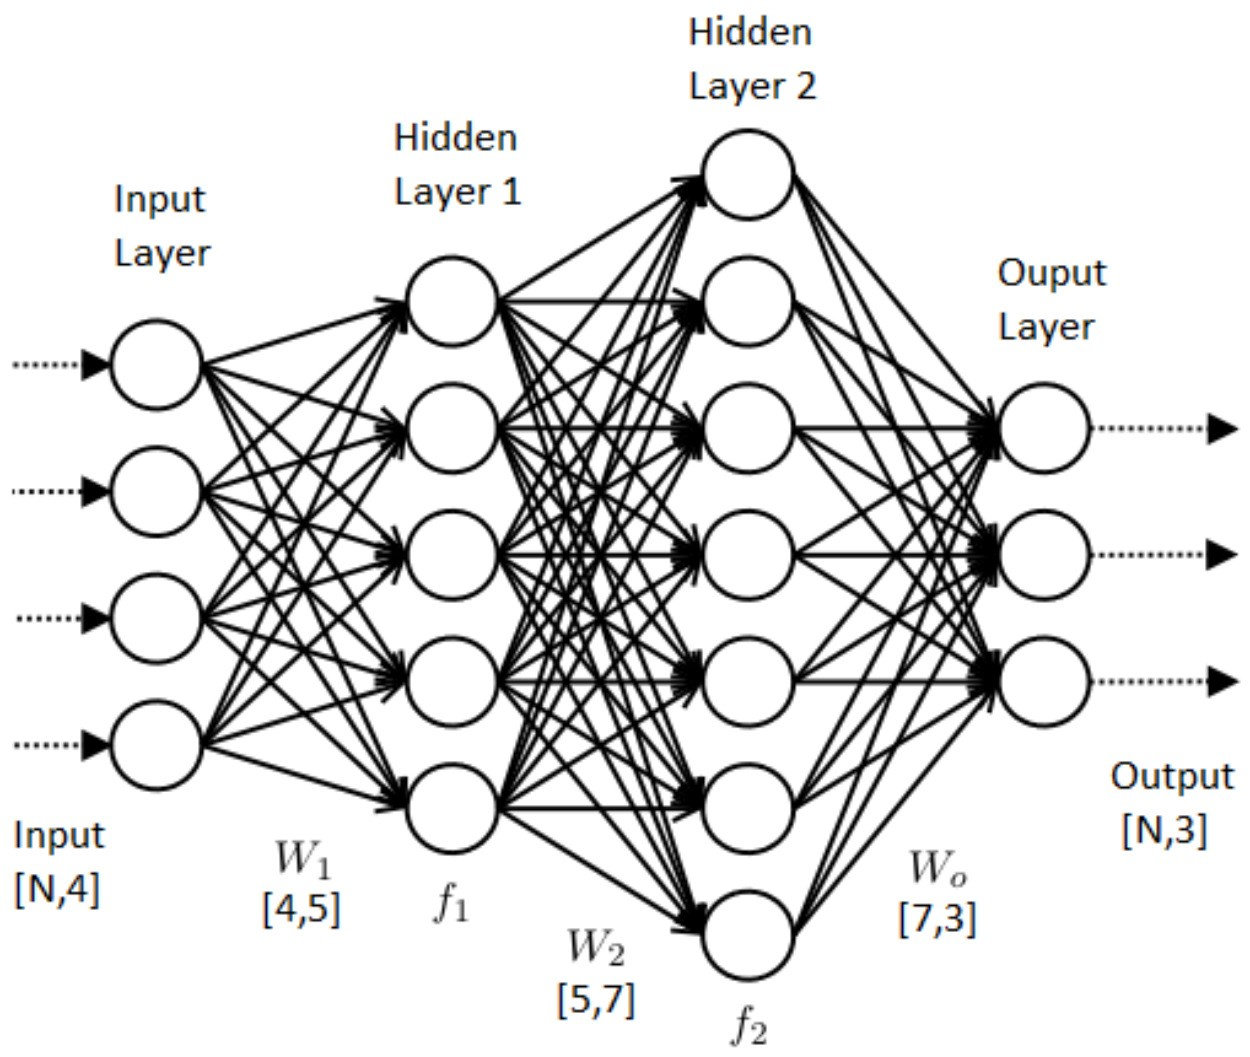
\includegraphics[width=8cm]{mlp.png}
    \caption{Simple multilayer perceptron.}
    \label{fig:2}
  \end{figure}

  The network iterates the input data through its hidden layer(s) (basically weighted sums are calculated followed by 
  so called ‘activation’ functions). In supervised approaches the weights are modified in the backpropagation process 
  in which a regularized cost function – reflecting the discrepancy between the inputs and the desired output – is tried 
  to be optimized. Depending on the input and output dimensionality and the design of the network it can have millions 
  of parameters which makes these calculations computationally expensive. This problem made the development of this 
  field a standstill until the rapid spread and improvement of GPUs started providing a huge advancement in 
  calculations.

  \subsubsection{Convolutional Networks}
  \label{sec:conv_nets}

  A class of deep neural networks are convolutional neural networks (CNN). The main design is the same as any other 
  networks (input, hidden layers, output). General CNNs use a set of convolutional layers followed by fully-connected 
  layers (all neurons in a layer are connected to every neuron in the preceding and following layers as seen on 
  \autoref{fig:2}) as hidden layers. Convolutional layers are used for representing small or high features in the data 
  with applying a convolutional operation to their input. It uses filters which are parts of the data with the same or 
  less dimension than the input. Using $k$ filters $k$ feature maps are generated.
  
  Attention is a mechanism which can be added to reach better results with the cost of more computational expenses 
  ~\cite{attention}. At a high-level attention can be described as giving the network the ability to learn which parts 
  are more important to focus on. It is commonly and successfully used at natural language processing tasks.

  \subsubsection{Long Short-Term Memory}
  \label{sec:lstm}

  LSTM networks \cite{lstm, lstm_colah} are a type of Recurrent Neural Netwoks (RNNs). The concept is to model the 
  aspect of human thinking that our understanding is not simply based on single samples of the world, rather we take 
  our observations on the past in consideration and based on that our reactions can be completely different. This is 
  achieved with three gates (with trainable parameters): the input-, the output- and the forget gate. The cell states 
  are passed through time and resetted when it is appropriate (exact number of timesteps or rule based, e.g. sentence 
  end). This report does not aim to fully explain the whole architecture, I just wanted to give a small insight.
  
  LSTMs have shown a huge advancement in sequence modeling and became widely used in the following years. However in the 
  recent years several studies stated and have shown that CNNs with attention can outperform these networks in a lot of 
  cases \cite{eval_conv_lstm, fall_rnn}.

  \subsubsection{Generative Adversarial Networks}
  \label{sec:gans}

  Generative adversarial networks (GAN) are deep neural architectures comprised of a generator and a discriminator 
  network (\autoref{fig:3}), introduced by Goodfellow et al. ~\cite{gan}. These two networks contest against each other 
  in the following way. The aim of the generator is to produce data indistinguishable of the real data and the 
  discriminator tries to classify whether its input was real data or fake, generated by the opposing network. The losses 
  of the networks are propagated back combined making both networks’ reward depending on both of their performance. This 
  means if the generator lacks competence the discriminator’s work will be easy thus the system will be incompatible of 
  solving the problem. The design and training of GANs is a complex task.

  \begin{figure}[tbh]
    \centering
    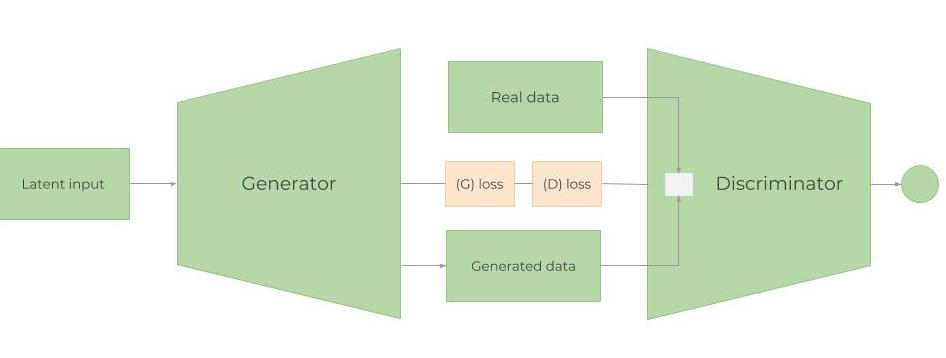
\includegraphics[width=12cm]{gan.jpg}
    \caption{GAN architecture example.}
    \label{fig:3}
  \end{figure}

\subsection{Starting point, previous works on this project}
\label{sec:prev_works}

At the start of the project I was no preceding work given and did not make any research on this topic before.

I started learning the theory of Deep Learning as part of the university course VITMAV45 and gained a well based 
knowledge on the subject to start with.

\newpage
%==================================================================
\begin{center}
  \section{Own work on project}
  \label{sec:work}
\end{center}

\subsection{Data}
\label{sec:data}

The project's first task was to find or collect a database to work with. On financial field the big and high frequency 
raw datasets which are precise enough can cost a lot of money (3000 USD+). There was no funding available so I collected 
my own raw data from Kraken (\url{www.kraken.com}) which is a US based cryptocurrency exchange. Kraken gives the 
opportunity to access live order book (and of course other) data through a REST- and a Websocket based API. 

In the training and evaluation process only ETH-EUR \footnote{Ethereum - Euro: Ethereum is an open-source, public, 
blockchain-based distributed computing platform and operating system featuring smart contract (scripting) functionality. 
- \textit{Wikipedia} } snapshots are used but for further research on universality and stationarity ~\cite{univ}. I save 
25 asset-pair's data in aggregate. For each currency 1 snapshot is querried every minute through REST API calls and the 
real-time order flow is recorded through the previosly mentioned Websocket API.  

The saved data is stored in CSV file format, \autoref{table:1} and \autoref{table:2} show the structure. Every 
asset-pair is saved to a separate folder and at the end of each day all buffer files (updates and snapshots) are 
compressed (I chose gzip compression) and saved into a separate file this way saving space and ensuring that the 
unexpected corruption of a file causes minimal data loss. The saving method also makes paralell datapreparation on 
multiple CPUs possible. The dataset contains entries from 15th March 2019.

\begin{table}[tbh]
  \centering
  \begin{tabular}{|l|l|}
    \hline
    Field              & Description \\
    \hline
    L1 Ask Price       & The price of the ask order at 1st level (best ask) \\
    \hline
    L1 Ask Volume      & The volume of the ask order at 1st level \\
    \hline
    L1 Ask Timestamp   & The last modification time of the ask order at 1st level \\
    \hline
    ... \\
    \hline
    L100 Ask Price     & The price of the ask order at 100th level \\
    \hline
    L100 Ask Volume    & The volume of the ask order at 100th level \\
    \hline
    L100 Ask Timestamp & The last modification time of the ask order at 100th level \\
    \hline
    L1 Bid Price       & The price of the bid order at 1st level (best bid) \\
    \hline
    L1 Bid Volume      & The volume of the bid order at 1st level \\
    \hline
    L1 Bid Timestamp   & The last modification time of the bid order at 1st level \\
    \hline
    ... \\
    \hline
    L100 Bid Price     & The price of the bid order at 100th level \\
    \hline
    L100 Bid Volume    & The volume of the bid order at 100th level \\
    \hline
    L100 Bid Timestamp & The last modification time of the bid order at 100th level \\
    \hline
    Timestamp          & The timestamp of the snapshot \\
    \hline
  \end{tabular}
  \caption{One snapshot (one row in snapshot files).}
  \label{table:1}
\end{table}

\begin{table}[tbh]
  \centering
  \begin{tabular}{|l|l|}
    \hline
    Field       & Description \\
    \hline
    AskOrBid    & The update type: 0 = ask, 1 = bid \\
    \hline
    Price       & The price of the order \\
    \hline
    Volume      & The volume of the order (0 means that the level is deleted)\\
    \hline
    Timestamp   & The last modification time \\
    \hline
  \end{tabular}
  \caption{One update (one row in update files).}
  \label{table:2}
\end{table}

  \subsubsection{Data preparation}
  \label{dataprep}

  I wrote a parameterizable python script to do the whole preprocessing. The following section explains the steps 
  executed by the generator.

  To train my models I chose to use 30 days of ETH-EUR limit order book history. The first step of the preprocessing is 
  to clean and reorder the update records to put them into an ascending flow. This is required because the Websocket API 
  not always sends the packets in the right order or a short loss of the network connection can also cause some 
  problems. At visualizing the data I also noticed that the API sometimes forwards updates with timestamps from few days 
  ago. Although I could not explain this behaviour I had to remove these entries. The next task was to process the 
  saved snapshots and create a full dataset which is saved to a single gzipped file. One parameter is which depth to 
  use and it is important to emphasize that this is the first operation as we calculate every metrics for the following 
  steps from the snapshots. Then these are followed by labelling and scaling operations which are explained in the next 
  two sections of this paper. Before feeding the consumed data into the used models the last step is to split it into 
  training, validation and test sets. By definition these sets must not have any intersections but since I use time 
  series data it was important to make one more constraint which is the datapoints in the train set must be prior to the 
  ones in validation and the same applies for validatin and test. This guaranties that the models learn to generalize 
  without seeing into the future. 

  To use it as an input each snapshot is needed to be converted to a one dimensional array. I use the prices and the 
  cumulative volumes from each level (the timesteps are dropped) in the ascending order of the price values (so 
  basically like on the top diagram of \autoref{fig:1}). 

  \subsubsection{Labels}
  \label{labels}

  For each snapshot the WAMP (\ref{eq:wamp}) or the VWAP (\ref{eq:vwap}) is calculated since these are used in further 
  steps. After this, we create the labels previously mentioned in \ref{sec:limit_order_book}. The research aims to 
  successfully predict the direction of the price movement using 3 categories: UP (1), DOWN (-1), NO\_MOVE (0). 
  Snapshots are labelled using the following technique, based on the method introduced in the work by Zihao Zhang et al. 
  (~\cite{deeplob}). Although trades aren't executed exactly at the WAMP or the VWAP, they are a good estimation since 
  they contain more information than the mid-price with also taking the volumes at the price levels in consideration. 
  As financial time series, especially high frequency limit order book metrics are highly stochastic, the comparison 
  between $WAMP_t$ and $WAMP_{t+1}$ would result noisy labels which are unable to compress bigger trends (here where the
  updates can happen on the scale of miliseconds this doesn't mean whole days, only minutes). I used a smoothing method 
  which I recall briefly in \autoref{eq:m_minus} and \autoref{eq:m_plus}. The first is the mean of the previous k –
  including the present one – (history), the second is the following k number of WAMPs (future). So k is the prediction 
  horizon. 

  \begin{equation}
    m\_(t) = \frac{1}{k}\sum_{i=0}^{k}p_{t-i}
    \label{eq:m_minus}
  \end{equation}

  \begin{equation}
    m_+(t) = \frac{1}{k}\sum_{i=1}^{k}p_{t+i}
    \label{eq:m_plus}
  \end{equation}

  The labels are decided based on a threshold which is calculated as multplying the volatility – calculated on the full 
  time period (history + future) – by $\alpha$, a hyperparameter. An example can be seen on \autoref{fig:4}. Red color 
  indicates the down, green the up and white the stationary labels.

  \begin{figure}[tbh]
    \centering
    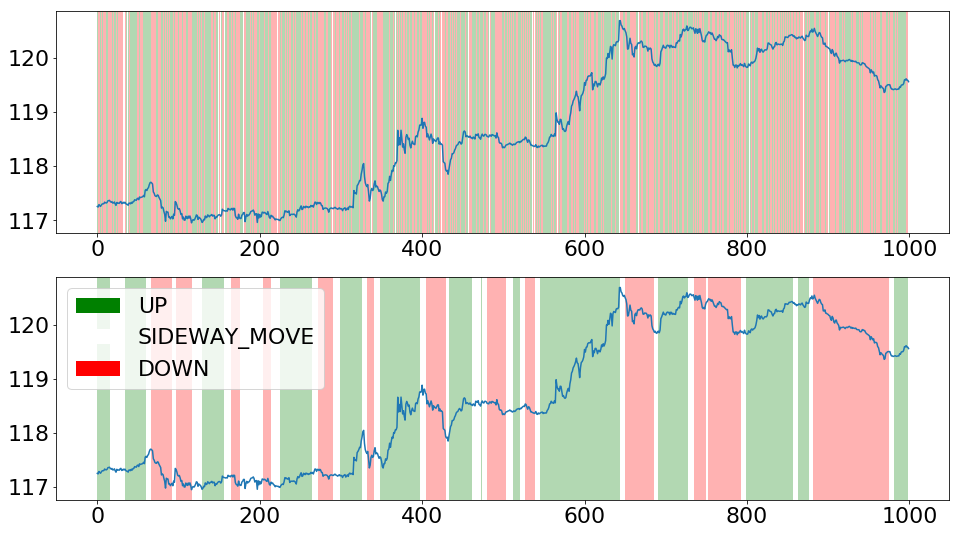
\includegraphics[width=10cm]{labels.png}
    \caption{Comparison between basic labeling and using the smoothing technique.}
    \label{fig:4}
  \end{figure}

  In my research i tried out 10, 20, 30, 50 and 100 as possible values for k and found 30 the ideal one and for 
  $\alpha$ 0.7 but these were selected based on my own opinion only.

  \subsubsection{Scaling}
  \label{scaling}

  After the labelling, the next step is to rescale the input (the snapshots as first approach). This is inevitable since 
  there are multiple reasons for it. One is that if we use multiple asset-pairs the numbers can be on different scales 
  e.g. the prices of Bitcoin and Ripple have a huge variance, this means we have to process them separately. The first 
  approach was to use the z-score standardization method. As financial time series have regime shifts a static 
  standardization would be inappropriate for a high frequency database over a considerable period of time, hence the 
  previous 3 day's mean and standard deviation was used to standardize the actual day's prices. As for the volumes my 
  first try was to simply normalize them, but a few tries showed that using the cumulative volumes at price levels 
  boosts performance. This is reasonable, as humans can also see more information from the cumulative volume chart than 
  from the normal diagram (\ref{fig:1}). This approach also partly solved the problem of the outliers which means that 
  some volumes were on an other scale than the othes in the same snapshot and they grew even bigger during the scaling 
  because they were too rare to effect the standard deviation which stayed a small number this way and enlarged the huge 
  numbers (as they were divided by them).

  For the recurrent neural networks a last task was to resample the dataset with the number of parameters as timestep to 
  create small series as inputs.

\subsection{Models}
\label{models}

In my work I used three methods as a starting-point (baseline) to see how a simple algorythm can solve this complex task 
and to have some results to which I can compare my future models. 

The first model is a very simple one, it uses a 
similar label calculation method as the labelling script except it only can use the past and present values to make it's 
prediction. It has two hyperparameters: alpha and k, alpha is used in the same way, k is the horizon. The 'mean baseline' 
calculates the mean of the VWAPS of the previous k snapshots and compares it to the VWAP of the snapshot in the present. 

The following two are logistic regression and random forest classification. I used the scikit-learn python library for 
both of them. Logistic regression is an approach to modelling the relationship between a dependent and one or more 
independent variables based on prior observations. It uses a logistic function to predict the target categorical 
dependent variable which is from the previously mentioned three categories (-1, 0, 1) in this cases.

Random forests is a supervised learning algorithm. It can be used both for classification and regression. A forest is 
comprised of trees. It creates decision trees on randomly selected data samples, gets prediction from each tree and 
selects the best solution by means of voting \cite{randomforest}.

The last approach (the first using neural networks) was a simple LSTM model. It's consists of a 1D Convolutional layer 
(with 32 filters, kernel size and strides both chosen to equal 2) to capture information at each order book level. The 
next is an LSTM layer with 64 cells and 0.4 dropout. This is followed by the fully connected structure which is a Dense 
layer with 100 cells ReLU as activation function and 0.2 dropout connected to another Dense layer with 3 cells that 
does the classification by applying softmax to the output.

\subsection{Results}
\label{sec:results}

Before showing the results it must be mentioned that predicting stock prices is an exceptionally hard task because of 
the highly stochastic behaviour of the maket, hence no good solution was publicated. The values follow some basic trends 
and some basic assumptions can be made based on limit order book snapshots but even a small imbalance or a simple news 
headline can make a great and unpredictable impact on exchanges since the complexity of human- and crowd behaviour. At 
high frequency financial data even a one percent deviation from the 'random guess' or baseline results can mean a huge 
change in profit. 

To visualize my results I use confusion matrixes because I think they are more representative than simply comparing 
percent values together.

\begin{table}[ht]
  \centering
  \begin{tabularx}{\columnwidth}{XX}
  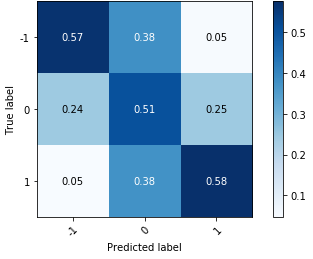
\includegraphics[width=\linewidth]{mb_results.png}
  \captionof{figure}{Mean baseline}\label{fig:5}
      &   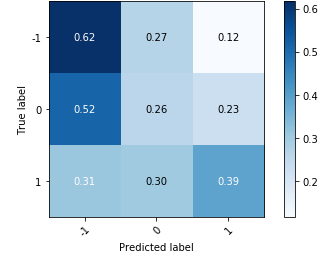
\includegraphics[width=\linewidth]{lr_results.png}   
          \captionof{figure}{Logistic regression}\label{fig:6}              \\
  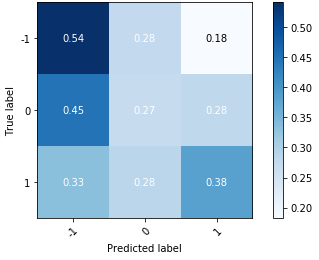
\includegraphics[width=0.45\columnwidth]{rf_results.png}
  \captionof{figure}{Random forest classification}\label{fig:7}
      &   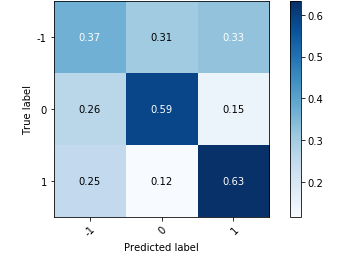
\includegraphics[width=\linewidth]{lstm_results.png} 
          \captionof{figure}{LSTM model}\label{fig:8}               
  \end{tabularx}
\end{table}%

For the predictions I used 30 days of ETH-EUR limit order book snapshots data which was divided into 80\% training and 
20\% test sets, in case of baseline models and 72\% training, 18\% validation and 10\% test data in case of neural 
networks. I collected price aggregated LOB snapshots with the depth of 100 but for my models I used only the best 30 
levels in this work to limit the number of parameters at first approaches. 

It is clear that the mean baseline (\autoref{fig:5}) gives surprisingly accurate predictions, however as I see it this 
is only because it uses a similar method as the labeling. Logistic regression (\autoref{fig:6}) and random forest 
classification (\autoref{fig:7}) can predict upward and downward movement fairly well but are unable to generalize in 
the stationary case. This can be caused by the fact that stationarity is highly subjective and based on personally 
chosen hyperparameters. LSTM (\autoref{fig:8}) shows an improvement to all models but the effect of misprediction of 
down labels needs further investigation.

\subsection{Summary}
\label{sec:summary}

In my work during the semester I succesfully managed to collect high frequency financial data with the help of a well
scalable system which can handle the everyday problems like loss of internet connection. I could visualize the gathered 
snapshots to help to get a deeper understanding on a financial topic which prevoiusly I was not familiar with. A complex 
data preparation process was applied to the raw data which made possible to implement or use some basic (mean baseline 
and regession techniques) and a neural network based model to serve as baseline for my further research on the field. 

The results confirmed my assumption on the topic that it is an especially complicated task with limited number of 
detailed enough publications. This part of the project mainly involved data collection and preparation as an 
introduction to the financial field of deep learning. I faced a well amount of problems and challenges with regard to 
hardware and software but with the help of my supervisor I could find a solution to most of them. Because of the short 
time and my other studies I could not complete all of the planned work but in the future work I would like to try more
complex architectures like Deep CNNs as well as GANs which was my original plan to do as I think they are really 
powerful models and I have only seen one research using them on this field but it was not the same approach (not for 
LOBs).

This, along with other studies showed that the topic is worth working on since it not only provides a lot of interesting 
barriers to overcome (which is not impossible in my opinion) but is promising to help to earn big profits.

\newpage
%==================================================================
\section{References}
\label{sec:references}

\begin{references}{9}

  \bibitem{univ} Justin Sirignano and Rama Cont (2018). 
  \emph{\href{https://arxiv.org/abs/1803.06917.pdf}{Universal features of price formation in financial markets: perspectives from Deep Learning}}

  \bibitem{attention} 
  \emph{\href{https://medium.com/syncedreview/a-brief-overview-of-attention-mechanism-13c578ba9129}{A Brief Overview of Attention Mechanism}}

  \bibitem{gan} Ian J. Goodfellow, Jean Pouget-Abadie, Mehdi Mirza, Bing Xu, David Warde-Farley, Sherjil Ozair, Aaron Courville, Yoshua Bengio (2014). 
  \emph{\href{http://papers.nips.cc/paper/5423-generative-adversarial-nets.pdf}{Generative Adversarial Nets}}

  \bibitem{lstm} Sepp Hochreiter, Jürgen Schmidhuber (1997). 
  \emph{\href{https://www.bioinf.jku.at/publications/older/2604.pdf}{Long Short-Term Memory}}

  \bibitem{lstm_colah} Christopher Olah (2015). 
  \emph{\href{https://colah.github.io/posts/2015-08-Understanding-LSTMs/}{Understanding LSTM Networks}}

  \bibitem{eval_conv_lstm} Shaojie Bai, J. Zico Kolter, Vladlen Koltun (2018). 
  \emph{\href{https://arxiv.org/pdf/1803.01271.pdf}{An Empirical Evaluation of Generic Convolutional and Recurrent Networks for Sequence Modeling}}
  
  \bibitem{fall_rnn} Eugenio Culurciello (2018). 
  \emph{\href{https://towardsdatascience.com/the-fall-of-rnn-lstm-2d1594c74ce0}{The fall of RNN / LSTM}}

  \bibitem{boris} 
  \emph{\href{https://github.com/borisbanushev/stockpredictionai}{Using the latest advancements in AI to predict stock market movements}}

  \bibitem{deeplob} Zihao Zhang, Stefan Zohren, and Stephen Roberts (2019). 
  \emph{\href{https://arxiv.org/abs/1803.06917.pdf}{DeepLOB: Deep Convolutional Neural Networks for Limit Order Books}}

  \bibitem{randomforest} Avinash Navlani (2018). 
  \emph{\href{https://www.datacamp.com/community/tutorials/random-forests-classifier-python}{Understanding Random Forests Classifiers in Python}}

\end{references}

%==================================================================
\subsection{Source code}
\label{sec:source_code}

The whole project's source code (except the crawler's) can be found on GitHub: \\ 
\url{https://github.com/tornermarton/SemesterProject} \\
On some topics a deeper insight/longer explanation can be found in the Markdown files under the docs folder. \\
Most of the images used here can be found in the Jupyter Notebooks which are publicated also in this repository. \\

\vspace{5mm}
\noindent{The following library served as a base for the crawler:} \\
\url{https://github.com/krakenfx/kraken-wsclient-py} 

\end{document} 

%%% Local Variables: 
%%% mode: latex 
%%% TeX-master: t 
%%% End:

